\documentclass{article}

\usepackage{arxiv}

\usepackage[utf8]{inputenc} % allow utf-8 input
\usepackage[T1]{fontenc}    % use 8-bit T1 fonts
\usepackage{lmodern}        % https://github.com/rstudio/rticles/issues/343
\usepackage{hyperref}       % hyperlinks
\usepackage{url}            % simple URL typesetting
\usepackage{booktabs}       % professional-quality tables
\usepackage{amsfonts}       % blackboard math symbols
\usepackage{nicefrac}       % compact symbols for 1/2, etc.
\usepackage{microtype}      % microtypography
\usepackage{graphicx}

\title{Vaccines at Velocity: Evaluating Potential Lives Saved by Earlier Vaccination in the COVID-19 Pandemic}

\author{
  }


% tightlist command for lists without linebreak
\providecommand{\tightlist}{%
  \setlength{\itemsep}{0pt}\setlength{\parskip}{0pt}}

% From pandoc table feature
\usepackage{longtable,booktabs,array}
\usepackage{calc} % for calculating minipage widths
% Correct order of tables after \paragraph or \subparagraph
\usepackage{etoolbox}
\makeatletter
\patchcmd\longtable{\par}{\if@noskipsec\mbox{}\fi\par}{}{}
\makeatother
% Allow footnotes in longtable head/foot
\IfFileExists{footnotehyper.sty}{\usepackage{footnotehyper}}{\usepackage{footnote}}
\makesavenoteenv{longtable}


\usepackage[authoryear,round]{natbib} \usepackage{authblk} \newcommand{\beginsupplement}{ \setcounter{table}{0} \renewcommand{\thetable}{S\arabic{table}} \setcounter{figure}{0} \renewcommand{\thefigure}{S\arabic{figure}}} \author[1]{Witold Więcek} \author[1]{David Johnston} \author[1]{Tomas Dulka} \author[1]{Danny Toomey} \author[1]{Enlli Lewis} \affil[1]{1Day Sooner, Delaware, United States}
\usepackage{float}
\usepackage{booktabs}
\usepackage{longtable}
\usepackage{array}
\usepackage{multirow}
\usepackage{wrapfig}
\usepackage{colortbl}
\usepackage{pdflscape}
\usepackage{tabu}
\usepackage{threeparttable}
\usepackage{threeparttablex}
\usepackage[normalem]{ulem}
\usepackage{makecell}
\usepackage{xcolor}
\begin{document}
\maketitle

\begin{figure}[H]

{\centering 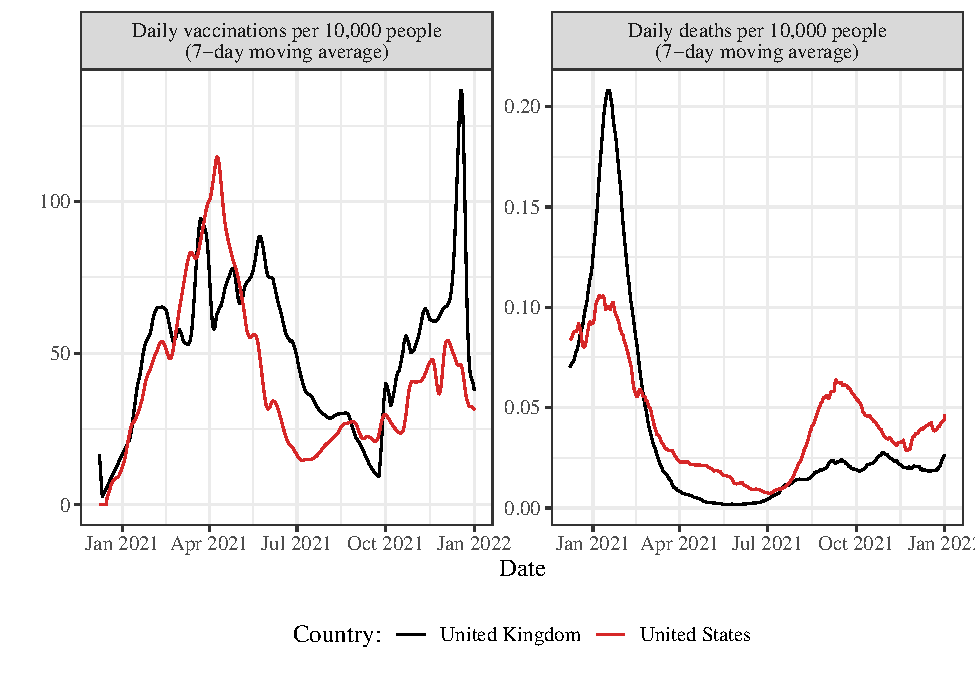
\includegraphics[height=0.4\textheight,]{_main_files/figure-latex/baseline-vacc-death-1}

}

\caption{Data on daily vaccinations and deaths in the UK and the US in 2021}\label{fig:baseline-vacc-death}
\end{figure}

\begin{table}

\caption{\label{tab:vaccinations-table}Total vaccinations under baseline and counterfactual scenarios}
\centering
\begin{tabular}[t]{lrrr}
\toprule
Counterfactual scenario & 2021-01-01 & 2021-04-01 & 2021-07-01\\
\midrule
\addlinespace[0.3em]
\multicolumn{4}{l}{\textbf{United Kingdom}}\\
\hspace{1em}Baseline & 1,462,757 & 36,015,897 & 78,366,737\\
\hspace{1em}Vaccines 30 days sooner & 5,868,579 & 44,767,107 & 83,205,069\\
\hspace{1em}Vaccines 60 days sooner & 17,132,520 & 59,668,154 & 89,288,187\\
\hspace{1em}Vaccines 90 days sooner & 30,302,416 & 73,937,217 & 93,731,611\\
\addlinespace[0.3em]
\multicolumn{4}{l}{\textbf{United States}}\\
\hspace{1em}Baseline & 4,521,988 & 172,124,225 & 347,123,032\\
\hspace{1em}Vaccines 30 days sooner & 23,889,241 & 238,670,399 & 357,876,350\\
\hspace{1em}Vaccines 60 days sooner & 56,107,462 & 289,245,438 & 372,702,522\\
\hspace{1em}Vaccines 90 days sooner & 56,107,489 & 289,245,510 & 376,955,754\\
\bottomrule
\end{tabular}
\end{table}

\begin{figure}[H]

{\centering 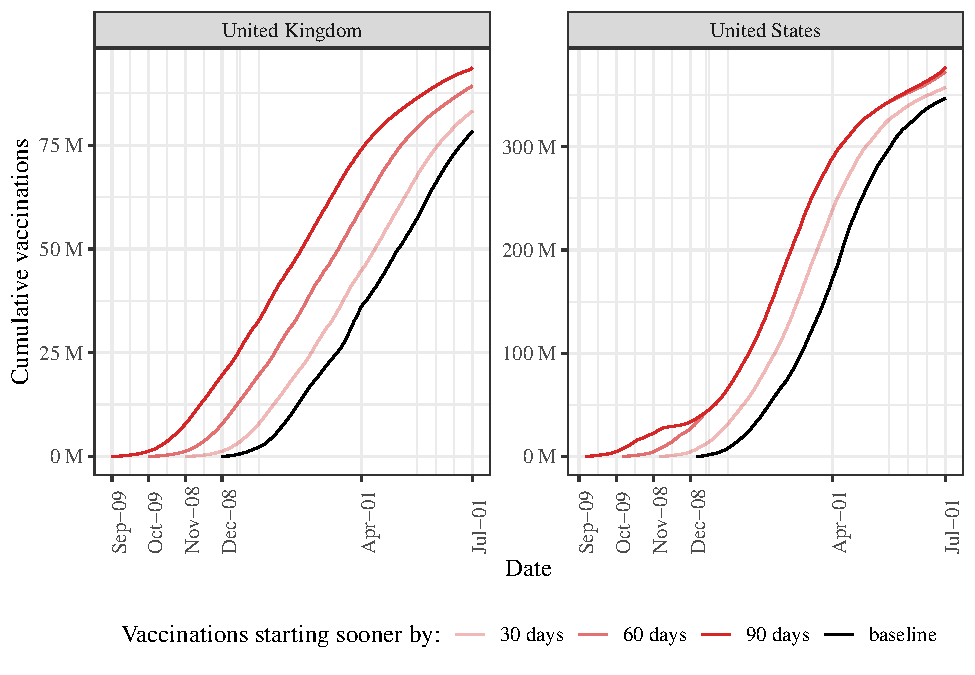
\includegraphics[height=0.4\textheight,]{_main_files/figure-latex/cumul-vacc-cfacts-1}

}

\caption{Cumulative vaccinations under baseline and counterfactual scenarios}\label{fig:cumul-vacc-cfacts}
\end{figure}

\begin{figure}[H]

{\centering 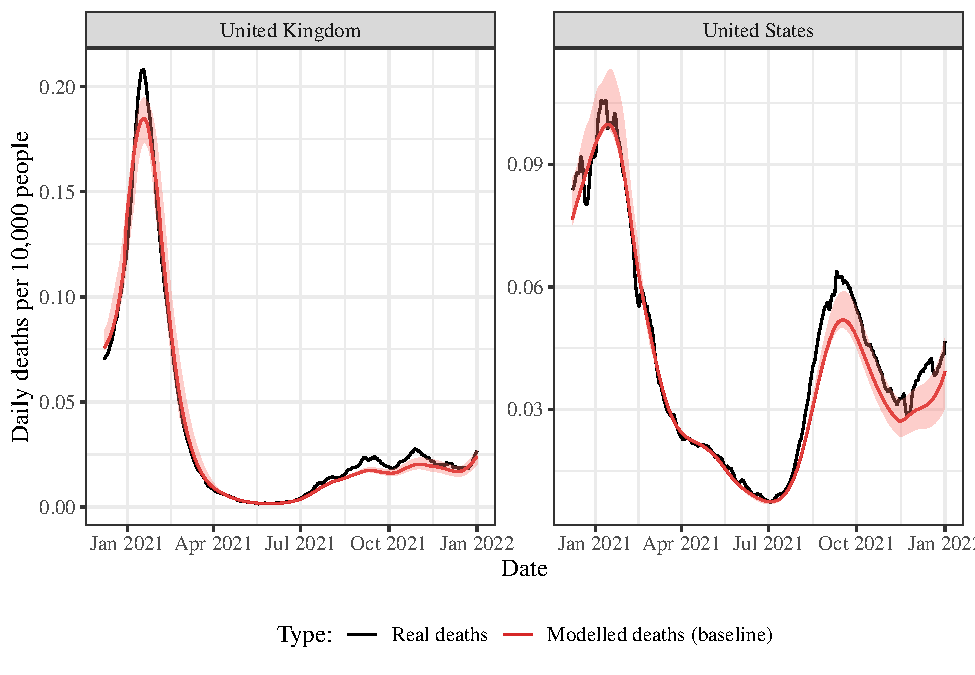
\includegraphics[height=0.4\textheight,]{_main_files/figure-latex/model-fit-deaths-1}

}

\caption{Comparison of real and modelled (baseline) deaths over time. Shaded areas indicate 95\% confidence interval.}\label{fig:model-fit-deaths}
\end{figure}

\begin{table}
\centering
\caption{\label{tab:deaths-averted-table}Total averted deaths under counterfactual scenarios, based on reported deaths. 95\% intervals are calculated over 100 simulation runs which vary vaccine parameters and duration of natural immunity (see Table S1 in Appendix for details). More details are given in Table S7.}
\centering
\fontsize{9}{11}\selectfont
\begin{tabular}[t]{lll}
\toprule
Counterfactual scenario & Deaths averted & Per 10,000 people\\
\midrule
\addlinespace[0.3em]
\multicolumn{3}{l}{\textbf{United Kingdom to April 2021}}\\
\hspace{1em}30 days sooner & 10,728 [6,627; 14,991] & 1.60 [0.99; 2.23]\\
\hspace{1em}60 days sooner & 29,922 [21,040; 43,472] & 4.46 [3.14; 6.48]\\
\hspace{1em}90 days sooner & 46,665 [37,966; 67,151] & 6.96 [5.66; 10.01]\\
\addlinespace[0.3em]
\multicolumn{3}{l}{\textbf{United Kingdom to July 2021}}\\
\hspace{1em}30 days sooner & 9,952 [6,026; 13,949] & 1.48 [0.90; 2.08]\\
\hspace{1em}60 days sooner & 30,516 [21,967; 43,452] & 4.55 [3.27; 6.48]\\
\hspace{1em}90 days sooner & 47,953 [39,529; 67,086] & 7.15 [5.89; 10.00]\\
\addlinespace[0.3em]
\multicolumn{3}{l}{\textbf{United Kingdom to Jan 2022}}\\
\hspace{1em}30 days sooner & 8,019 [-2,350; 17,181] & 1.20 [-0.35; 2.56]\\
\hspace{1em}60 days sooner & 41,389 [35,940; 49,167] & 6.17 [5.36; 7.33]\\
\hspace{1em}90 days sooner & 65,485 [60,730; 77,178] & 9.76 [9.05; 11.51]\\
\addlinespace[0.3em]
\multicolumn{3}{l}{\textbf{United States to April 2021}}\\
\hspace{1em}30 days sooner & 35,207 [25,342; 63,091] & 1.06 [0.76; 1.90]\\
\hspace{1em}60 days sooner & 87,601 [67,671; 143,053] & 2.64 [2.04; 4.32]\\
\hspace{1em}90 days sooner & 107,134 [86,198; 167,087] & 3.23 [2.60; 5.04]\\
\addlinespace[0.3em]
\multicolumn{3}{l}{\textbf{United States to July 2021}}\\
\hspace{1em}30 days sooner & 53,342 [45,493; 73,576] & 1.61 [1.37; 2.22]\\
\hspace{1em}60 days sooner & 115,895 [99,725; 152,977] & 3.50 [3.01; 4.61]\\
\hspace{1em}90 days sooner & 132,919 [117,226; 173,179] & 4.01 [3.54; 5.22]\\
\addlinespace[0.3em]
\multicolumn{3}{l}{\textbf{United States to Jan 2022}}\\
\hspace{1em}30 days sooner & 45,196 [3,320; 101,695] & 1.36 [0.10; 3.07]\\
\hspace{1em}60 days sooner & 120,655 [-32,178; 221,714] & 3.64 [-0.97; 6.69]\\
\hspace{1em}90 days sooner & 175,230 [56,961; 255,219] & 5.29 [1.72; 7.70]\\
\bottomrule
\end{tabular}
\end{table}

\begin{figure}[H]

{\centering 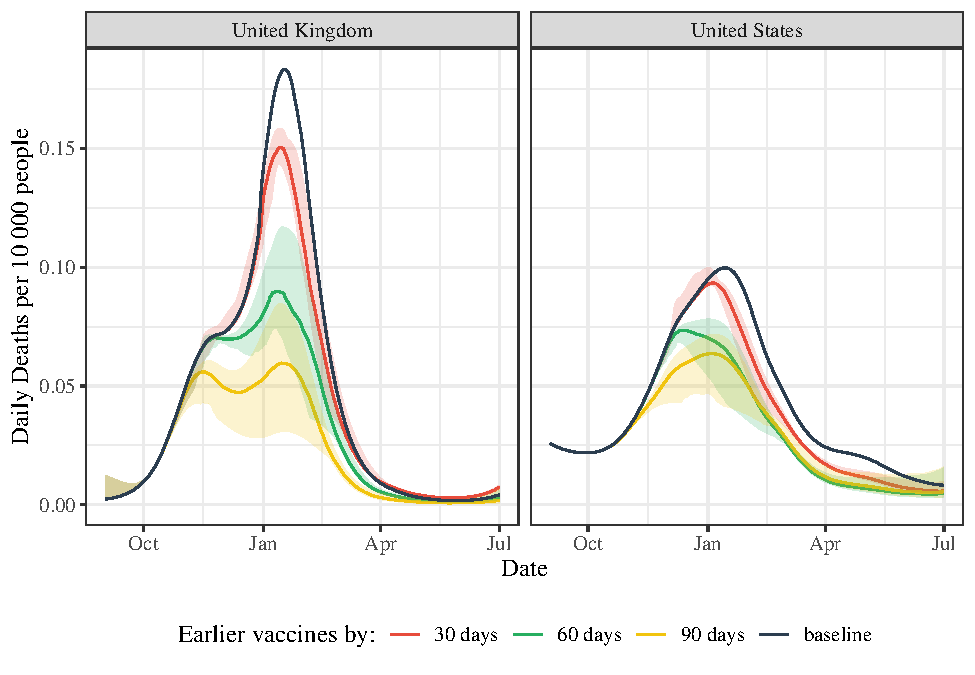
\includegraphics[height=0.4\textheight,]{_main_files/figure-latex/deaths-averted-plot-1}

}

\caption{Daily deaths under baseline and counterfactual scenarios. Shaded area indicates 95\% confidence interval. Cumulative reductions are shown in the Appendix.}\label{fig:deaths-averted-plot}
\end{figure}

\appendix


\setcounter{table}{0} \renewcommand{\thetable}{S\arabic{table}} \setcounter{figure}{0} \renewcommand{\thefigure}{S\arabic{figure}}

\begin{figure}[H]

{\centering 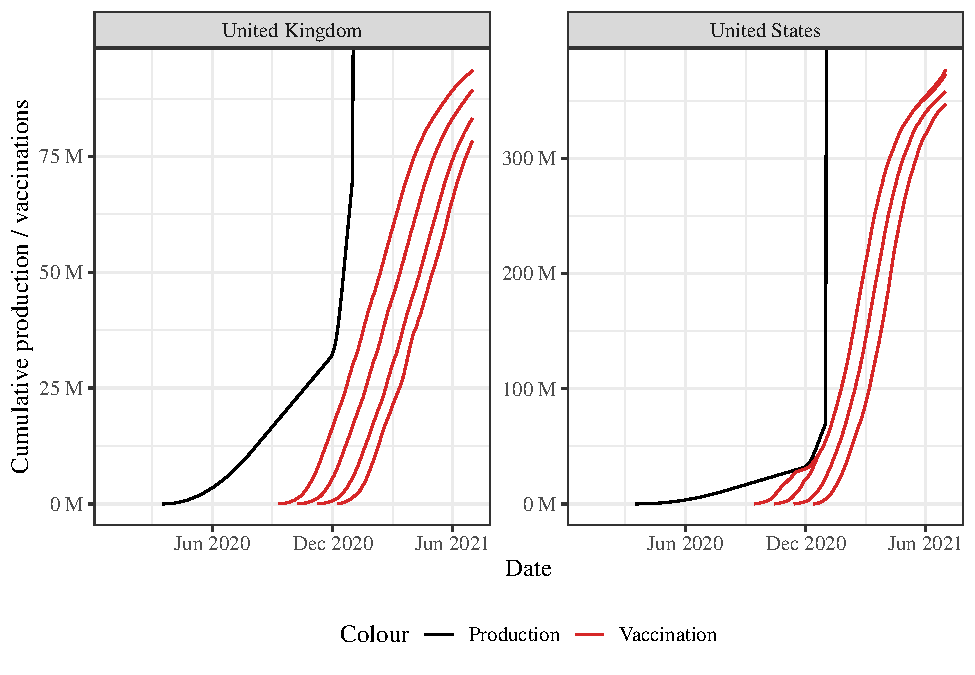
\includegraphics[height=0.4\textheight,]{_main_files/figure-latex/prod-cap-1}

}

\caption{Cumulative vaccine production and distribution in the UK and the US under counterfactual and baseline scenarios. Four lines in red are different acceleration factors, from baseline up to 90 days earlier approval.}\label{fig:prod-cap}
\end{figure}

\begin{table}

\caption{\label{tab:trajectory-sampling-parameters}Distributions from which parameters are sampled. The parameters $\alpha_e^P, \beta_e^P$ are shape parameters for vaccine platform $P$ with associated efficacy $e$ (see text for additional details). The parameters $\alpha_d, \beta_d$ are shape and rate parameters for distribution of vaccine durations, determined by fitting an antibody decay curve to vaccine efficacies. $\mathrm{rescale}(\cdot, f_{min}, f_{med}, f_{max})$ is a function that maps $0$ to $f_{min}$, $0.5$ to $f_{med}$ and $1$ to $f_{max}$, linearly interpolating between each. $f_{min}, f_{med}, f_{max}$ are respectively the minimum, median, and maximum estimates of age-adjusted infection fatality.}
\centering
\begin{tabular}[t]{ll}
\toprule
Parameter & Distribution\\
\midrule
Vaccine efficacy, $V$ & $V\sim \mathrm{Beta}(\alpha_{e}^P, \beta_{e}^P), P = \mathrm{vaccine\; platform})$\\
Vaccine immunity duration, $D$ & $\frac{1}{\mathrm{Gamma}(\alpha_{d}, \beta_d)}$\\
Infection fatality rate with vaccination, $F$ & $F = \mathrm{rescale}(X,f_{min}, f_{med}, f_{max}), \quad X\sim \mathrm{Beta}(2,2)$\\
Natural immunity duration, $R$ & $R = \mathrm{Gamma}(20, 4/73)$\\
\bottomrule
\end{tabular}
\end{table}

\begin{table}

\caption{\label{tab:vaccine-efficacy}Model parameters - central estimates of vaccine efficacy}
\centering
\begin{tabular}[t]{llll}
\toprule
Vaccine type & Doses & Strain & Protection against infection\\
\midrule
mRNA & 1 & Wild & 63\%\\
mRNA & 2 & Wild & 86\%\\
mRNA & 1 & Delta & 36\%\\
mRNA & 2 & Delta & 88\%\\
mRNA & 1 & Omicron & 0\%\\
mRNA & 2 & Omicron & 13.6\%\\
mRNA & 3 & Omicron & 65\%\\
Adenovirus & Partial & Wild & 64\%\\
Adenovirus & Full & Wild & 77\%\\
Adenovirus & Partial & Delta & 30\%\\
Adenovirus & Full & Delta & 67\%\\
\bottomrule
\end{tabular}
\end{table}

\begin{table}

\caption{\label{tab:onward}Assumed relative transmissibility of infection by vaccinated individuals compared to unvaccinated}
\centering
\begin{tabular}[t]{ll}
\toprule
Doses & Protection from onward transmission\\
\midrule
1 dose (not wanted) & 27\%\\
2 doses (not wanted) & 27\%\\
2 doses (waned) & 0\%\\
3 doses (not wanted) & 30\%\\
3 doses (waned stage 1) & 10\%\\
3 doses (waned stage 2) & 5\%\\
\bottomrule
\end{tabular}
\end{table}

\section{Supplementary Figures and Tables}\label{supplementary-figures-and-tables}

\begin{table}
\centering
\caption{\label{tab:deaths-averted-table-full}Total averted deaths under counterfactual scenarios, based on reported deaths. 95\% intervals are calculated over 100 simulation runs which vary vaccine parameters and duration of natural immunity (see Table S1 for details). This table provides additional results for Table 2.}
\centering
\fontsize{9}{11}\selectfont
\begin{tabular}[t]{llllr}
\toprule
Counterfactual scenario & Deaths averted & Per 10,000 people & Baseline deaths & Averted/baseline\\
\midrule
\addlinespace[0.3em]
\multicolumn{5}{l}{\textbf{United Kingdom to April 2021}}\\
\hspace{1em}30 days sooner & 10,728 [6,627; 14,991] & 1.60 [0.99; 2.23] & 69,808 & 0.15\\
\hspace{1em}60 days sooner & 29,922 [21,040; 43,472] & 4.46 [3.14; 6.48] & 84,124 & 0.36\\
\hspace{1em}90 days sooner & 46,665 [37,966; 67,151] & 6.96 [5.66; 10.01] & 92,216 & 0.51\\
\addlinespace[0.3em]
\multicolumn{5}{l}{\textbf{United Kingdom to July 2021}}\\
\hspace{1em}30 days sooner & 9,952 [6,026; 13,949] & 1.48 [0.90; 2.08] & 71,862 & 0.14\\
\hspace{1em}60 days sooner & 30,516 [21,967; 43,452] & 4.55 [3.27; 6.48] & 86,178 & 0.35\\
\hspace{1em}90 days sooner & 47,953 [39,529; 67,086] & 7.15 [5.89; 10.00] & 94,270 & 0.51\\
\addlinespace[0.3em]
\multicolumn{5}{l}{\textbf{United Kingdom to Jan 2022}}\\
\hspace{1em}30 days sooner & 8,019 [-2,350; 17,181] & 1.20 [-0.35; 2.56] & 95,018 & 0.08\\
\hspace{1em}60 days sooner & 41,389 [35,940; 49,167] & 6.17 [5.36; 7.33] & 109,334 & 0.38\\
\hspace{1em}90 days sooner & 65,485 [60,730; 77,178] & 9.76 [9.05; 11.51] & 117,427 & 0.56\\
\addlinespace[0.3em]
\multicolumn{5}{l}{\textbf{United States to April 2021}}\\
\hspace{1em}30 days sooner & 35,207 [25,342; 63,091] & 1.06 [0.76; 1.90] & 310,390 & 0.11\\
\hspace{1em}60 days sooner & 87,601 [67,671; 143,053] & 2.64 [2.04; 4.32] & 341,910 & 0.26\\
\hspace{1em}90 days sooner & 107,134 [86,198; 167,087] & 3.23 [2.60; 5.04] & 364,108 & 0.29\\
\addlinespace[0.3em]
\multicolumn{5}{l}{\textbf{United States to July 2021}}\\
\hspace{1em}30 days sooner & 53,342 [45,493; 73,576] & 1.61 [1.37; 2.22] & 358,199 & 0.15\\
\hspace{1em}60 days sooner & 115,895 [99,725; 152,977] & 3.50 [3.01; 4.61] & 389,719 & 0.30\\
\hspace{1em}90 days sooner & 132,919 [117,226; 173,179] & 4.01 [3.54; 5.22] & 411,917 & 0.32\\
\addlinespace[0.3em]
\multicolumn{5}{l}{\textbf{United States to Jan 2022}}\\
\hspace{1em}30 days sooner & 45,196 [3,320; 101,695] & 1.36 [0.10; 3.07] & 583,198 & 0.08\\
\hspace{1em}60 days sooner & 120,655 [-32,178; 221,714] & 3.64 [-0.97; 6.69] & 614,719 & 0.20\\
\hspace{1em}90 days sooner & 175,230 [56,961; 255,219] & 5.29 [1.72; 7.70] & 636,916 & 0.28\\
\bottomrule
\end{tabular}
\end{table}

\begin{figure}[H]

{\centering 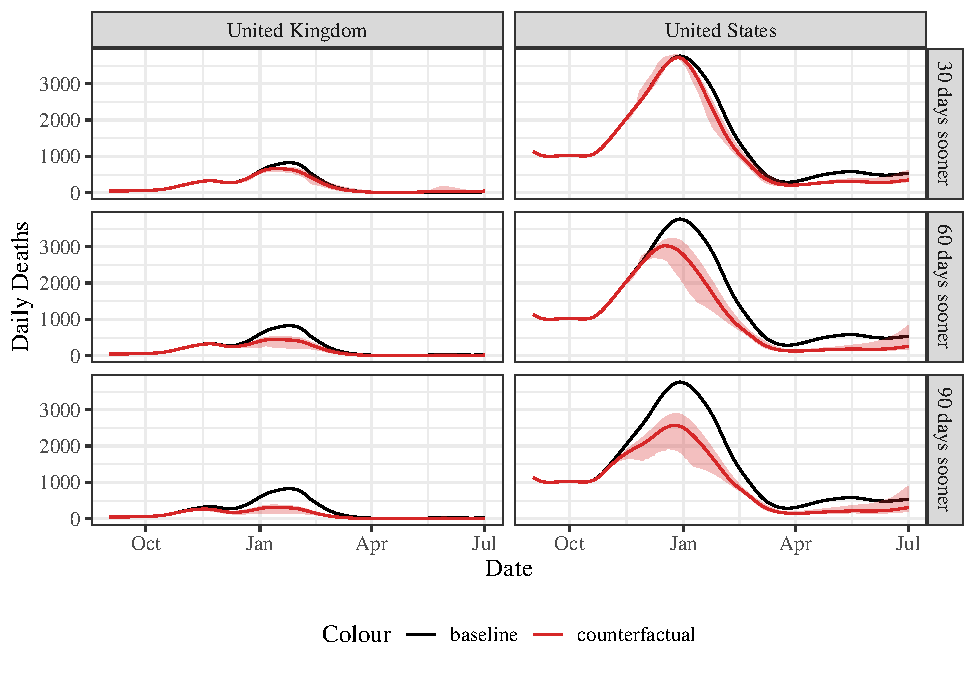
\includegraphics[height=0.4\textheight,]{_main_files/figure-latex/reported-deaths-averted-plot-1}

}

\caption{Reported deaths for each counerfactual scenario compared to baseline reported deaths. Shaded area indicates 95\% confidence interval.}\label{fig:reported-deaths-averted-plot}
\end{figure}

\begin{figure}[H]

{\centering 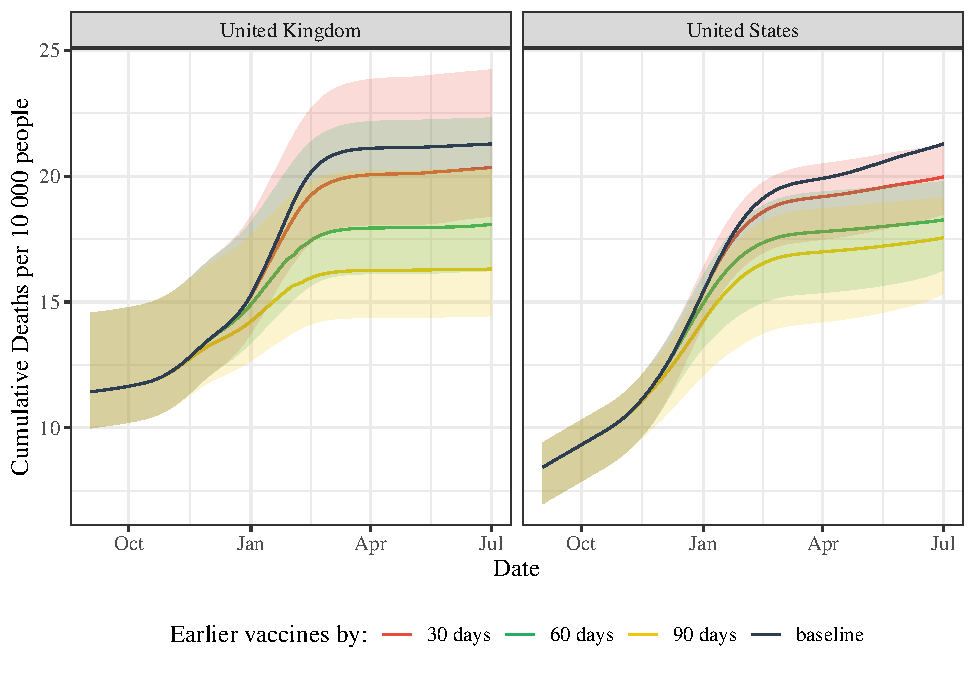
\includegraphics[height=0.4\textheight,]{_main_files/figure-latex/cumulative-deaths-1}

}

\caption{Cumulative deaths under baseline and counterfactual scenarios. Shaded area indicates 95\% confidence interval}\label{fig:cumulative-deaths}
\end{figure}

\begin{table}
\centering
\caption{\label{tab:deaths-averted-table-d90}How would outcomes change if vaccination demand were 10\% lower}
\centering
\fontsize{7}{9}\selectfont
\begin{tabular}[t]{llllr}
\toprule
Counterfactual scenario & Deaths averted & Per 10,000 people & Baseline deaths & Averted/baseline\\
\midrule
\addlinespace[0.3em]
\multicolumn{5}{l}{\textbf{United Kingdom to April 2021}}\\
\hspace{1em}30 days sooner & 9,208 [5,600; 12,392] & 1.37 [0.83; 1.85] & 69,808 & 0.13\\
\hspace{1em}60 days sooner & 27,691 [19,208; 39,888] & 4.13 [2.86; 5.95] & 84,124 & 0.33\\
\hspace{1em}90 days sooner & 44,061 [35,169; 65,092] & 6.57 [5.24; 9.70] & 92,216 & 0.48\\
\addlinespace[0.3em]
\multicolumn{5}{l}{\textbf{United Kingdom to July 2021}}\\
\hspace{1em}30 days sooner & 7,596 [4,228; 10,548] & 1.13 [0.63; 1.57] & 71,862 & 0.11\\
\hspace{1em}60 days sooner & 27,735 [19,660; 39,240] & 4.13 [2.93; 5.85] & 86,178 & 0.32\\
\hspace{1em}90 days sooner & 44,886 [36,445; 64,154] & 6.69 [5.43; 9.56] & 94,270 & 0.48\\
\addlinespace[0.3em]
\multicolumn{5}{l}{\textbf{United Kingdom to Jan 2022}}\\
\hspace{1em}30 days sooner & -14,878 [-76,737; 7,384] & -2.22 [-11.44; 1.10] & 95,018 & -0.16\\
\hspace{1em}60 days sooner & 9,691 [-14,387; 29,963] & 1.44 [-2.14; 4.47] & 109,334 & 0.09\\
\hspace{1em}90 days sooner & 39,790 [31,759; 56,986] & 5.93 [4.73; 8.50] & 117,427 & 0.34\\
\addlinespace[0.3em]
\multicolumn{5}{l}{\textbf{United States to April 2021}}\\
\hspace{1em}30 days sooner & 30,365 [21,689; 55,905] & 0.92 [0.65; 1.69] & 310,390 & 0.10\\
\hspace{1em}60 days sooner & 80,279 [61,435; 133,348] & 2.42 [1.85; 4.02] & 341,910 & 0.23\\
\hspace{1em}90 days sooner & 98,186 [79,051; 155,592] & 2.96 [2.38; 4.69] & 364,108 & 0.27\\
\addlinespace[0.3em]
\multicolumn{5}{l}{\textbf{United States to July 2021}}\\
\hspace{1em}30 days sooner & 40,202 [33,996; 58,510] & 1.21 [1.03; 1.77] & 358,199 & 0.11\\
\hspace{1em}60 days sooner & 101,539 [87,394; 134,921] & 3.06 [2.64; 4.07] & 389,719 & 0.26\\
\hspace{1em}90 days sooner & 115,630 [104,019; 153,078] & 3.49 [3.14; 4.62] & 411,917 & 0.28\\
\addlinespace[0.3em]
\multicolumn{5}{l}{\textbf{United States to Jan 2022}}\\
\hspace{1em}30 days sooner & -49,504 [-90,132; 32,157] & -1.49 [-2.72; 0.97] & 583,198 & -0.08\\
\hspace{1em}60 days sooner & 23,485 [-71,246; 90,271] & 0.71 [-2.15; 2.72] & 614,719 & 0.04\\
\hspace{1em}90 days sooner & 80,385 [6,176; 143,145] & 2.42 [0.19; 4.32] & 636,916 & 0.13\\
\bottomrule
\end{tabular}
\end{table}

\begin{table}
\centering
\caption{\label{tab:deaths-averted-table-d95}How would outcomes change if vaccination demand were 5\% lower?}
\centering
\fontsize{7}{9}\selectfont
\begin{tabular}[t]{llllr}
\toprule
Counterfactual scenario & Deaths averted & Per 10,000 people & Baseline deaths & Averted/baseline\\
\midrule
\addlinespace[0.3em]
\multicolumn{5}{l}{\textbf{United Kingdom to April 2021}}\\
\hspace{1em}30 days sooner & 9,977 [6,147; 13,710] & 1.49 [0.92; 2.04] & 69,808 & 0.14\\
\hspace{1em}60 days sooner & 28,797 [20,136; 41,753] & 4.29 [3.00; 6.22] & 84,124 & 0.34\\
\hspace{1em}90 days sooner & 45,385 [36,575; 66,146] & 6.77 [5.45; 9.86] & 92,216 & 0.49\\
\addlinespace[0.3em]
\multicolumn{5}{l}{\textbf{United Kingdom to July 2021}}\\
\hspace{1em}30 days sooner & 8,802 [5,190; 12,319] & 1.31 [0.77; 1.84] & 71,862 & 0.12\\
\hspace{1em}60 days sooner & 29,150 [20,849; 41,441] & 4.35 [3.11; 6.18] & 86,178 & 0.34\\
\hspace{1em}90 days sooner & 46,465 [38,005; 65,640] & 6.93 [5.67; 9.79] & 94,270 & 0.49\\
\addlinespace[0.3em]
\multicolumn{5}{l}{\textbf{United Kingdom to Jan 2022}}\\
\hspace{1em}30 days sooner & -4,209 [-36,876; 11,673] & -0.63 [-5.50; 1.74] & 95,018 & -0.04\\
\hspace{1em}60 days sooner & 26,578 [20,035; 38,228] & 3.96 [2.99; 5.70] & 109,334 & 0.24\\
\hspace{1em}90 days sooner & 56,491 [48,152; 68,647] & 8.42 [7.18; 10.23] & 117,427 & 0.48\\
\addlinespace[0.3em]
\multicolumn{5}{l}{\textbf{United States to April 2021}}\\
\hspace{1em}30 days sooner & 32,814 [23,533; 59,598] & 0.99 [0.71; 1.80] & 310,390 & 0.11\\
\hspace{1em}60 days sooner & 84,004 [64,622; 138,347] & 2.53 [1.95; 4.17] & 341,910 & 0.25\\
\hspace{1em}90 days sooner & 102,734 [82,735; 161,675] & 3.10 [2.50; 4.88] & 364,108 & 0.28\\
\addlinespace[0.3em]
\multicolumn{5}{l}{\textbf{United States to July 2021}}\\
\hspace{1em}30 days sooner & 47,149 [40,040; 66,332] & 1.42 [1.21; 2.00] & 358,199 & 0.13\\
\hspace{1em}60 days sooner & 108,980 [93,903; 144,340] & 3.29 [2.83; 4.35] & 389,719 & 0.28\\
\hspace{1em}90 days sooner & 125,010 [110,971; 163,692] & 3.77 [3.35; 4.94] & 411,917 & 0.30\\
\addlinespace[0.3em]
\multicolumn{5}{l}{\textbf{United States to Jan 2022}}\\
\hspace{1em}30 days sooner & 2,578 [-33,216; 46,710] & 0.08 [-1.00; 1.41] & 583,198 & 0.00\\
\hspace{1em}60 days sooner & 74,985 [-50,099; 147,926] & 2.26 [-1.51; 4.46] & 614,719 & 0.12\\
\hspace{1em}90 days sooner & 128,759 [38,392; 191,873] & 3.88 [1.16; 5.79] & 636,916 & 0.20\\
\bottomrule
\end{tabular}
\end{table}

\begin{table}
\centering
\caption{\label{tab:deaths-averted-table-doubleboost}How would US outcomes change if boosters were adopted at twice the actual rate?}
\centering
\fontsize{7}{9}\selectfont
\begin{tabular}[t]{llllr}
\toprule
Counterfactual scenario & Deaths averted & Per 10,000 people & Baseline deaths & Averted/baseline\\
\midrule
\addlinespace[0.3em]
\multicolumn{5}{l}{\textbf{United Kingdom to April 2021}}\\
\hspace{1em}30 days sooner & 6,923 [5,482; 10,845] & 1.03 [0.82; 1.62] & 47,105 & 0.15\\
\hspace{1em}60 days sooner & 19,055 [16,178; 29,735] & 2.84 [2.41; 4.43] & 56,206 & 0.34\\
\hspace{1em}90 days sooner & 31,079 [27,164; 39,334] & 4.63 [4.05; 5.86] & 61,709 & 0.50\\
\addlinespace[0.3em]
\multicolumn{5}{l}{\textbf{United Kingdom to July 2021}}\\
\hspace{1em}30 days sooner & 6,256 [4,739; 9,296] & 0.93 [0.71; 1.39] & 48,329 & 0.13\\
\hspace{1em}60 days sooner & 19,513 [16,767; 29,889] & 2.91 [2.50; 4.46] & 57,430 & 0.34\\
\hspace{1em}90 days sooner & 32,028 [27,911; 39,828] & 4.77 [4.16; 5.94] & 62,933 & 0.51\\
\addlinespace[0.3em]
\multicolumn{5}{l}{\textbf{United Kingdom to Jan 2022}}\\
\hspace{1em}30 days sooner & 6,240 [-4,129; 19,744] & 0.93 [-0.62; 2.94] & 84,531 & 0.07\\
\hspace{1em}60 days sooner & 38,111 [33,509; 41,848] & 5.68 [5.00; 6.24] & 93,631 & 0.41\\
\hspace{1em}90 days sooner & 62,520 [54,053; 66,192] & 9.32 [8.06; 9.87] & 99,134 & 0.63\\
\addlinespace[0.3em]
\multicolumn{5}{l}{\textbf{United States to April 2021}}\\
\hspace{1em}30 days sooner & 24,552 [17,774; 40,322] & 0.74 [0.54; 1.22] & 296,895 & 0.08\\
\hspace{1em}60 days sooner & 72,072 [54,156; 111,904] & 2.17 [1.63; 3.38] & 338,137 & 0.21\\
\hspace{1em}90 days sooner & 97,464 [76,963; 149,298] & 2.94 [2.32; 4.50] & 368,555 & 0.26\\
\addlinespace[0.3em]
\multicolumn{5}{l}{\textbf{United States to July 2021}}\\
\hspace{1em}30 days sooner & 43,602 [38,591; 52,063] & 1.32 [1.16; 1.57] & 342,236 & 0.13\\
\hspace{1em}60 days sooner & 100,332 [86,295; 126,194] & 3.03 [2.60; 3.81] & 383,478 & 0.26\\
\hspace{1em}90 days sooner & 124,047 [107,995; 157,820] & 3.74 [3.26; 4.76] & 413,895 & 0.30\\
\addlinespace[0.3em]
\multicolumn{5}{l}{\textbf{United States to Jan 2022}}\\
\hspace{1em}30 days sooner & 51,045 [-36,144; 124,584] & 1.54 [-1.09; 3.76] & 647,587 & 0.08\\
\hspace{1em}60 days sooner & 160,448 [-65,642; 272,969] & 4.84 [-1.98; 8.23] & 688,829 & 0.23\\
\hspace{1em}90 days sooner & 254,410 [96,230; 327,270] & 7.67 [2.90; 9.87] & 719,246 & 0.35\\
\bottomrule
\end{tabular}
\end{table}

\begin{table}
\centering
\caption{\label{tab:reported-deaths-averted-table}Averted deaths calculated on the basis of a model fit to excess deaths}
\centering
\fontsize{7}{9}\selectfont
\begin{tabular}[t]{llllr}
\toprule
Counterfactual scenario & Deaths averted & Per 10,000 people & Baseline deaths & Averted/baseline\\
\midrule
\addlinespace[0.3em]
\multicolumn{5}{l}{\textbf{United Kingdom to April 2021}}\\
\hspace{1em}30 days sooner & 6,923 [5,482; 10,845] & 1.03 [0.82; 1.62] & 47,105 & 0.15\\
\hspace{1em}60 days sooner & 19,055 [16,178; 29,735] & 2.84 [2.41; 4.43] & 56,206 & 0.34\\
\hspace{1em}90 days sooner & 31,079 [27,164; 39,334] & 4.63 [4.05; 5.86] & 61,709 & 0.50\\
\addlinespace[0.3em]
\multicolumn{5}{l}{\textbf{United Kingdom to July 2021}}\\
\hspace{1em}30 days sooner & 6,256 [4,739; 9,296] & 0.93 [0.71; 1.39] & 48,329 & 0.13\\
\hspace{1em}60 days sooner & 19,513 [16,767; 29,889] & 2.91 [2.50; 4.46] & 57,430 & 0.34\\
\hspace{1em}90 days sooner & 32,028 [27,911; 39,828] & 4.77 [4.16; 5.94] & 62,933 & 0.51\\
\addlinespace[0.3em]
\multicolumn{5}{l}{\textbf{United Kingdom to Jan 2022}}\\
\hspace{1em}30 days sooner & 6,240 [-4,129; 19,744] & 0.93 [-0.62; 2.94] & 84,531 & 0.07\\
\hspace{1em}60 days sooner & 38,111 [33,509; 41,848] & 5.68 [5.00; 6.24] & 93,631 & 0.41\\
\hspace{1em}90 days sooner & 62,520 [54,053; 66,192] & 9.32 [8.06; 9.87] & 99,134 & 0.63\\
\addlinespace[0.3em]
\multicolumn{5}{l}{\textbf{United States to April 2021}}\\
\hspace{1em}30 days sooner & 24,555 [17,788; 40,319] & 0.74 [0.54; 1.22] & 296,896 & 0.08\\
\hspace{1em}60 days sooner & 72,049 [54,157; 111,909] & 2.17 [1.63; 3.38] & 338,138 & 0.21\\
\hspace{1em}90 days sooner & 97,463 [76,943; 149,291] & 2.94 [2.32; 4.50] & 368,555 & 0.26\\
\addlinespace[0.3em]
\multicolumn{5}{l}{\textbf{United States to July 2021}}\\
\hspace{1em}30 days sooner & 43,592 [38,604; 52,077] & 1.31 [1.16; 1.57] & 342,242 & 0.13\\
\hspace{1em}60 days sooner & 100,312 [86,296; 126,203] & 3.03 [2.60; 3.81] & 383,484 & 0.26\\
\hspace{1em}90 days sooner & 124,026 [107,939; 157,734] & 3.74 [3.26; 4.76] & 413,901 & 0.30\\
\addlinespace[0.3em]
\multicolumn{5}{l}{\textbf{United States to Jan 2022}}\\
\hspace{1em}30 days sooner & 25,971 [-42,451; 98,451] & 0.78 [-1.28; 2.97] & 677,535 & 0.04\\
\hspace{1em}60 days sooner & 97,944 [-92,089; 245,497] & 2.95 [-2.78; 7.41] & 718,776 & 0.14\\
\hspace{1em}90 days sooner & 175,542 [12,829; 293,716] & 5.30 [0.39; 8.86] & 749,194 & 0.23\\
\bottomrule
\end{tabular}
\end{table}

\newpage

\section{Sensitivity To Model Parameters}\label{sensitivity-to-model-parameters}

\begin{table}
\centering
\caption{\label{tab:deaths-averted-table-vei}Sensitivity to average vaccine efficacy against infection (VEI)}
\centering
\fontsize{7}{9}\selectfont
\begin{tabular}[t]{lrlllr}
\toprule
Counterfactual scenario & Average VEI & Deaths averted & Per 10,000 people & Baseline deaths & Averted/baseline\\
\midrule
\addlinespace[0.3em]
\multicolumn{6}{l}{\textbf{UK to April 2021}}\\
\hspace{1em}30 days sooner & 0.30 & 8,061 [6,347; 10,880] & 1.20 [0.95; 1.62] & 47,754 & 0.17\\
\hspace{1em}30 days sooner & 0.38 & 6,419 [4,622; 9,976] & 0.96 [0.69; 1.49] & 47,047 & 0.14\\
\hspace{1em}60 days sooner & 0.30 & 19,879 [18,575; 29,871] & 2.96 [2.77; 4.45] & 56,846 & 0.35\\
\hspace{1em}60 days sooner & 0.38 & 17,818 [13,944; 23,680] & 2.66 [2.08; 3.53] & 56,139 & 0.32\\
\hspace{1em}90 days sooner & 0.30 & 31,483 [30,466; 39,411] & 4.69 [4.54; 5.88] & 62,353 & 0.50\\
\hspace{1em}90 days sooner & 0.38 & 29,800 [25,156; 35,487] & 4.44 [3.75; 5.29] & 61,639 & 0.48\\
\addlinespace[0.3em]
\multicolumn{6}{l}{\textbf{UK to July 2021}}\\
\hspace{1em}30 days sooner & 0.30 & 7,446 [5,518; 9,483] & 1.11 [0.82; 1.41] & 48,933 & 0.15\\
\hspace{1em}30 days sooner & 0.38 & 5,836 [4,017; 8,401] & 0.87 [0.60; 1.25] & 48,250 & 0.12\\
\hspace{1em}60 days sooner & 0.30 & 20,196 [19,312; 30,408] & 3.01 [2.88; 4.53] & 58,025 & 0.35\\
\hspace{1em}60 days sooner & 0.38 & 18,389 [14,642; 24,177] & 2.74 [2.18; 3.60] & 57,342 & 0.32\\
\hspace{1em}90 days sooner & 0.30 & 32,517 [31,104; 40,573] & 4.85 [4.64; 6.05] & 63,532 & 0.51\\
\hspace{1em}90 days sooner & 0.38 & 30,797 [26,345; 36,503] & 4.59 [3.93; 5.44] & 62,842 & 0.49\\
\addlinespace[0.3em]
\multicolumn{6}{l}{\textbf{UK to Jan 2022}}\\
\hspace{1em}30 days sooner & 0.30 & 10,665 [-3,118; 20,343] & 1.59 [-0.46; 3.03] & 85,020 & 0.13\\
\hspace{1em}30 days sooner & 0.38 & 5,753 [-2,082; 13,126] & 0.86 [-0.31; 1.96] & 84,503 & 0.07\\
\hspace{1em}60 days sooner & 0.30 & 37,894 [33,999; 41,226] & 5.65 [5.07; 6.15] & 94,112 & 0.40\\
\hspace{1em}60 days sooner & 0.38 & 37,344 [33,305; 39,994] & 5.57 [4.96; 5.96] & 93,595 & 0.40\\
\hspace{1em}90 days sooner & 0.30 & 58,649 [55,605; 65,452] & 8.74 [8.29; 9.76] & 99,619 & 0.59\\
\hspace{1em}90 days sooner & 0.38 & 61,365 [56,441; 63,909] & 9.15 [8.41; 9.53] & 99,095 & 0.62\\
\addlinespace[0.3em]
\multicolumn{6}{l}{\textbf{US to April 2021}}\\
\hspace{1em}30 days sooner & 0.31 & 25,697 [18,251; 46,089] & 0.78 [0.55; 1.39] & 296,988 & 0.09\\
\hspace{1em}30 days sooner & 0.41 & 29,162 [18,193; 34,581] & 0.88 [0.55; 1.04] & 295,836 & 0.10\\
\hspace{1em}60 days sooner & 0.31 & 74,073 [55,613; 119,134] & 2.23 [1.68; 3.59] & 338,235 & 0.22\\
\hspace{1em}60 days sooner & 0.41 & 82,195 [55,103; 97,149] & 2.48 [1.66; 2.93] & 337,172 & 0.24\\
\hspace{1em}90 days sooner & 0.31 & 98,347 [78,265; 150,635] & 2.97 [2.36; 4.54] & 368,658 & 0.27\\
\hspace{1em}90 days sooner & 0.41 & 108,366 [76,943; 125,315] & 3.27 [2.32; 3.78] & 367,629 & 0.29\\
\addlinespace[0.3em]
\multicolumn{6}{l}{\textbf{US to July 2021}}\\
\hspace{1em}30 days sooner & 0.31 & 43,560 [38,545; 56,405] & 1.31 [1.16; 1.70] & 342,272 & 0.13\\
\hspace{1em}30 days sooner & 0.41 & 45,709 [38,840; 49,358] & 1.38 [1.17; 1.49] & 341,237 & 0.13\\
\hspace{1em}60 days sooner & 0.31 & 100,856 [86,891; 133,113] & 3.04 [2.62; 4.02] & 383,520 & 0.26\\
\hspace{1em}60 days sooner & 0.41 & 107,427 [86,996; 119,326] & 3.24 [2.62; 3.60] & 382,572 & 0.28\\
\hspace{1em}90 days sooner & 0.31 & 122,609 [108,301; 159,218] & 3.70 [3.27; 4.80] & 413,943 & 0.30\\
\hspace{1em}90 days sooner & 0.41 & 129,324 [107,937; 143,007] & 3.90 [3.26; 4.31] & 413,030 & 0.31\\
\addlinespace[0.3em]
\multicolumn{6}{l}{\textbf{US to Jan 2022}}\\
\hspace{1em}30 days sooner & 0.31 & 14,368 [-15,276; 88,749] & 0.43 [-0.46; 2.68] & 677,223 & 0.02\\
\hspace{1em}30 days sooner & 0.41 & 15,872 [-19,292; 83,746] & 0.48 [-0.58; 2.53] & 676,539 & 0.02\\
\hspace{1em}60 days sooner & 0.31 & 97,113 [-34,020; 228,267] & 2.93 [-1.03; 6.89] & 718,470 & 0.14\\
\hspace{1em}60 days sooner & 0.41 & 52,676 [-23,546; 226,750] & 1.59 [-0.71; 6.84] & 717,875 & 0.07\\
\hspace{1em}90 days sooner & 0.31 & 174,699 [61,595; 279,568] & 5.27 [1.86; 8.43] & 748,893 & 0.23\\
\hspace{1em}90 days sooner & 0.41 & 134,634 [77,458; 276,178] & 4.06 [2.34; 8.33] & 748,332 & 0.18\\
\bottomrule
\end{tabular}
\end{table}
\begin{table}
\centering
\caption{\label{tab:deaths-averted-table-durV}Sensitivity to duration of vaccine acquired immunity (DVI)}
\centering
\fontsize{7}{9}\selectfont
\begin{tabular}[t]{lrlllr}
\toprule
Counterfactual scenario & Average DVI & Deaths averted & Per 10,000 people & Baseline deaths & Averted/baseline\\
\midrule
\addlinespace[0.3em]
\multicolumn{6}{l}{\textbf{UK to April 2021}}\\
\hspace{1em}30 days sooner & 307 & 6,714 [5,833; 7,661] & 1.00 [0.87; 1.14] & 47,200 & 0.14\\
\hspace{1em}30 days sooner & 311 & 7,731 [5,861; 11,161] & 1.15 [0.87; 1.66] & 47,581 & 0.16\\
\hspace{1em}60 days sooner & 307 & 18,401 [17,170; 19,475] & 2.74 [2.56; 2.90] & 56,302 & 0.33\\
\hspace{1em}60 days sooner & 311 & 19,835 [16,898; 28,831] & 2.96 [2.52; 4.30] & 56,695 & 0.35\\
\hspace{1em}90 days sooner & 307 & 30,356 [28,784; 31,251] & 4.53 [4.29; 4.66] & 61,807 & 0.49\\
\hspace{1em}90 days sooner & 311 & 31,177 [28,748; 38,715] & 4.65 [4.29; 5.77] & 62,209 & 0.50\\
\addlinespace[0.3em]
\multicolumn{6}{l}{\textbf{UK to July 2021}}\\
\hspace{1em}30 days sooner & 307 & 6,067 [5,116; 6,892] & 0.90 [0.76; 1.03] & 48,481 & 0.13\\
\hspace{1em}30 days sooner & 311 & 7,092 [5,130; 10,198] & 1.06 [0.76; 1.52] & 48,759 & 0.15\\
\hspace{1em}60 days sooner & 307 & 18,998 [17,896; 19,932] & 2.83 [2.67; 2.97] & 57,583 & 0.33\\
\hspace{1em}60 days sooner & 311 & 20,188 [17,492; 29,002] & 3.01 [2.61; 4.32] & 57,873 & 0.35\\
\hspace{1em}90 days sooner & 307 & 31,184 [29,588; 32,469] & 4.65 [4.41; 4.84] & 63,088 & 0.49\\
\hspace{1em}90 days sooner & 311 & 31,860 [29,786; 39,116] & 4.75 [4.44; 5.83] & 63,386 & 0.50\\
\addlinespace[0.3em]
\multicolumn{6}{l}{\textbf{UK to Jan 2022}}\\
\hspace{1em}30 days sooner & 307 & 5,361 [-787; 6,472] & 0.80 [-0.12; 0.96] & 84,738 & 0.06\\
\hspace{1em}30 days sooner & 311 & 10,736 [869; 16,592] & 1.60 [0.13; 2.47] & 84,932 & 0.13\\
\hspace{1em}60 days sooner & 307 & 39,224 [36,623; 40,855] & 5.85 [5.46; 6.09] & 93,841 & 0.42\\
\hspace{1em}60 days sooner & 311 & 37,621 [33,808; 40,629] & 5.61 [5.04; 6.06] & 94,046 & 0.40\\
\hspace{1em}90 days sooner & 307 & 63,745 [60,012; 64,470] & 9.50 [8.95; 9.61] & 99,345 & 0.64\\
\hspace{1em}90 days sooner & 311 & 60,462 [54,577; 63,479] & 9.01 [8.14; 9.46] & 99,560 & 0.61\\
\addlinespace[0.3em]
\multicolumn{6}{l}{\textbf{US to April 2021}}\\
\hspace{1em}30 days sooner & 316 & 20,583 [18,676; 33,860] & 0.62 [0.56; 1.02] & 297,055 & 0.07\\
\hspace{1em}30 days sooner & 319 & 27,058 [19,662; 41,157] & 0.82 [0.59; 1.24] & 296,599 & 0.09\\
\hspace{1em}60 days sooner & 316 & 62,213 [57,741; 96,328] & 1.88 [1.74; 2.91] & 338,265 & 0.18\\
\hspace{1em}60 days sooner & 319 & 77,933 [59,667; 111,234] & 2.35 [1.80; 3.36] & 337,870 & 0.23\\
\hspace{1em}90 days sooner & 316 & 86,836 [81,229; 123,798] & 2.62 [2.45; 3.73] & 368,675 & 0.24\\
\hspace{1em}90 days sooner & 319 & 103,449 [83,147; 143,490] & 3.12 [2.51; 4.33] & 368,297 & 0.28\\
\addlinespace[0.3em]
\multicolumn{6}{l}{\textbf{US to July 2021}}\\
\hspace{1em}30 days sooner & 316 & 40,960 [39,705; 48,919] & 1.24 [1.20; 1.48] & 342,380 & 0.12\\
\hspace{1em}30 days sooner & 319 & 45,377 [40,193; 51,652] & 1.37 [1.21; 1.56] & 341,852 & 0.13\\
\hspace{1em}60 days sooner & 316 & 93,289 [89,688; 118,305] & 2.81 [2.71; 3.57] & 383,589 & 0.24\\
\hspace{1em}60 days sooner & 319 & 105,808 [91,011; 125,079] & 3.19 [2.75; 3.77] & 383,123 & 0.28\\
\hspace{1em}90 days sooner & 316 & 116,022 [110,928; 140,186] & 3.50 [3.35; 4.23] & 414,000 & 0.28\\
\hspace{1em}90 days sooner & 319 & 127,677 [113,003; 152,312] & 3.85 [3.41; 4.59] & 413,550 & 0.31\\
\addlinespace[0.3em]
\multicolumn{6}{l}{\textbf{US to Jan 2022}}\\
\hspace{1em}30 days sooner & 316 & 20,707 [-15,079; 79,958] & 0.62 [-0.45; 2.41] & 677,770 & 0.03\\
\hspace{1em}30 days sooner & 319 & 15,258 [-16,320; 56,716] & 0.46 [-0.49; 1.71] & 676,626 & 0.02\\
\hspace{1em}60 days sooner & 316 & 104,249 [-19,159; 221,533] & 3.14 [-0.58; 6.68] & 718,979 & 0.14\\
\hspace{1em}60 days sooner & 319 & 78,202 [-19,587; 182,171] & 2.36 [-0.59; 5.50] & 717,897 & 0.11\\
\hspace{1em}90 days sooner & 316 & 181,420 [79,392; 275,209] & 5.47 [2.39; 8.30] & 749,389 & 0.24\\
\hspace{1em}90 days sooner & 319 & 162,718 [82,397; 243,528] & 4.91 [2.49; 7.35] & 748,323 & 0.22\\
\bottomrule
\end{tabular}
\end{table}
\begin{table}
\centering
\caption{\label{tab:deaths-averted-table-durR}Sensitivity to duration of naturally acquired immunity (DNI)}
\centering
\fontsize{7}{9}\selectfont
\begin{tabular}[t]{lrlllr}
\toprule
Counterfactual scenario & Average DNI & Deaths averted & Per 10,000 people & Baseline deaths & Averted/baseline\\
\midrule
\addlinespace[0.3em]
\multicolumn{6}{l}{\textbf{UK to April 2021}}\\
\hspace{1em}30 days sooner & 171 & 7,940 [7,229; 8,894] & 1.18 [1.08; 1.33] & 46,675 & 0.17\\
\hspace{1em}30 days sooner & 319 & 7,683 [5,537; 11,360] & 1.15 [0.83; 1.69] & 46,773 & 0.16\\
\hspace{1em}60 days sooner & 171 & 20,006 [19,364; 21,734] & 2.98 [2.89; 3.24] & 55,785 & 0.36\\
\hspace{1em}60 days sooner & 319 & 20,103 [16,604; 29,202] & 3.00 [2.48; 4.35] & 55,870 & 0.36\\
\hspace{1em}90 days sooner & 171 & 31,619 [30,232; 33,380] & 4.71 [4.51; 4.98] & 61,293 & 0.52\\
\hspace{1em}90 days sooner & 319 & 32,204 [28,936; 39,145] & 4.80 [4.31; 5.84] & 61,377 & 0.52\\
\addlinespace[0.3em]
\multicolumn{6}{l}{\textbf{UK to July 2021}}\\
\hspace{1em}30 days sooner & 171 & 7,255 [6,512; 8,208] & 1.08 [0.97; 1.22] & 47,801 & 0.15\\
\hspace{1em}30 days sooner & 319 & 6,856 [4,800; 10,289] & 1.02 [0.72; 1.53] & 47,939 & 0.14\\
\hspace{1em}60 days sooner & 171 & 20,451 [19,718; 22,096] & 3.05 [2.94; 3.29] & 56,911 & 0.36\\
\hspace{1em}60 days sooner & 319 & 20,569 [17,415; 29,393] & 3.07 [2.60; 4.38] & 57,036 & 0.36\\
\hspace{1em}90 days sooner & 171 & 32,466 [30,934; 34,093] & 4.84 [4.61; 5.08] & 62,419 & 0.52\\
\hspace{1em}90 days sooner & 319 & 33,061 [29,772; 39,589] & 4.93 [4.44; 5.90] & 62,543 & 0.53\\
\addlinespace[0.3em]
\multicolumn{6}{l}{\textbf{UK to Jan 2022}}\\
\hspace{1em}30 days sooner & 171 & 8,930 [-852; 10,687] & 1.33 [-0.13; 1.59] & 84,060 & 0.11\\
\hspace{1em}30 days sooner & 319 & 7,329 [-4,160; 16,951] & 1.09 [-0.62; 2.53] & 84,050 & 0.09\\
\hspace{1em}60 days sooner & 171 & 37,675 [36,263; 41,374] & 5.62 [5.41; 6.17] & 93,170 & 0.40\\
\hspace{1em}60 days sooner & 319 & 37,663 [34,557; 41,777] & 5.61 [5.15; 6.23] & 93,148 & 0.40\\
\hspace{1em}90 days sooner & 171 & 61,709 [59,875; 65,294] & 9.20 [8.93; 9.73] & 98,678 & 0.63\\
\hspace{1em}90 days sooner & 319 & 60,833 [54,561; 65,168] & 9.07 [8.13; 9.71] & 98,654 & 0.62\\
\addlinespace[0.3em]
\multicolumn{6}{l}{\textbf{US to April 2021}}\\
\hspace{1em}30 days sooner & 164 & 24,384 [19,583; 40,876] & 0.74 [0.59; 1.23] & 296,247 & 0.08\\
\hspace{1em}30 days sooner & 328 & 21,593 [18,193; 39,528] & 0.65 [0.55; 1.19] & 297,087 & 0.07\\
\hspace{1em}60 days sooner & 164 & 71,497 [58,307; 110,472] & 2.16 [1.76; 3.33] & 337,478 & 0.21\\
\hspace{1em}60 days sooner & 328 & 64,643 [55,103; 109,230] & 1.95 [1.66; 3.30] & 338,340 & 0.19\\
\hspace{1em}90 days sooner & 164 & 99,670 [79,617; 142,683] & 3.01 [2.40; 4.30] & 367,880 & 0.27\\
\hspace{1em}90 days sooner & 328 & 89,065 [76,943; 143,587] & 2.69 [2.32; 4.33] & 368,792 & 0.24\\
\addlinespace[0.3em]
\multicolumn{6}{l}{\textbf{US to July 2021}}\\
\hspace{1em}30 days sooner & 164 & 42,844 [39,400; 51,747] & 1.29 [1.19; 1.56] & 341,461 & 0.13\\
\hspace{1em}30 days sooner & 328 & 41,403 [38,840; 51,544] & 1.25 [1.17; 1.55] & 342,572 & 0.12\\
\hspace{1em}60 days sooner & 164 & 99,234 [89,253; 125,167] & 2.99 [2.69; 3.78] & 382,692 & 0.26\\
\hspace{1em}60 days sooner & 328 & 94,713 [86,996; 125,403] & 2.86 [2.62; 3.78] & 383,826 & 0.25\\
\hspace{1em}90 days sooner & 164 & 123,793 [109,555; 152,754] & 3.73 [3.30; 4.61] & 413,094 & 0.30\\
\hspace{1em}90 days sooner & 328 & 117,389 [107,937; 154,139] & 3.54 [3.26; 4.65] & 414,278 & 0.28\\
\addlinespace[0.3em]
\multicolumn{6}{l}{\textbf{US to Jan 2022}}\\
\hspace{1em}30 days sooner & 164 & 35,607 [256; 100,555] & 1.07 [0.01; 3.03] & 677,232 & 0.05\\
\hspace{1em}30 days sooner & 328 & 12,896 [-29,811; 83,805] & 0.39 [-0.90; 2.53] & 677,844 & 0.02\\
\hspace{1em}60 days sooner & 164 & 121,773 [10,496; 243,476] & 3.67 [0.32; 7.34] & 718,463 & 0.17\\
\hspace{1em}60 days sooner & 328 & 101,608 [-67,484; 226,829] & 3.07 [-2.04; 6.84] & 719,098 & 0.14\\
\hspace{1em}90 days sooner & 164 & 194,125 [104,565; 291,236] & 5.86 [3.15; 8.79] & 748,865 & 0.26\\
\hspace{1em}90 days sooner & 328 & 174,009 [24,027; 276,591] & 5.25 [0.72; 8.34] & 749,550 & 0.23\\
\bottomrule
\end{tabular}
\end{table}
\begin{figure}[H]

{\centering 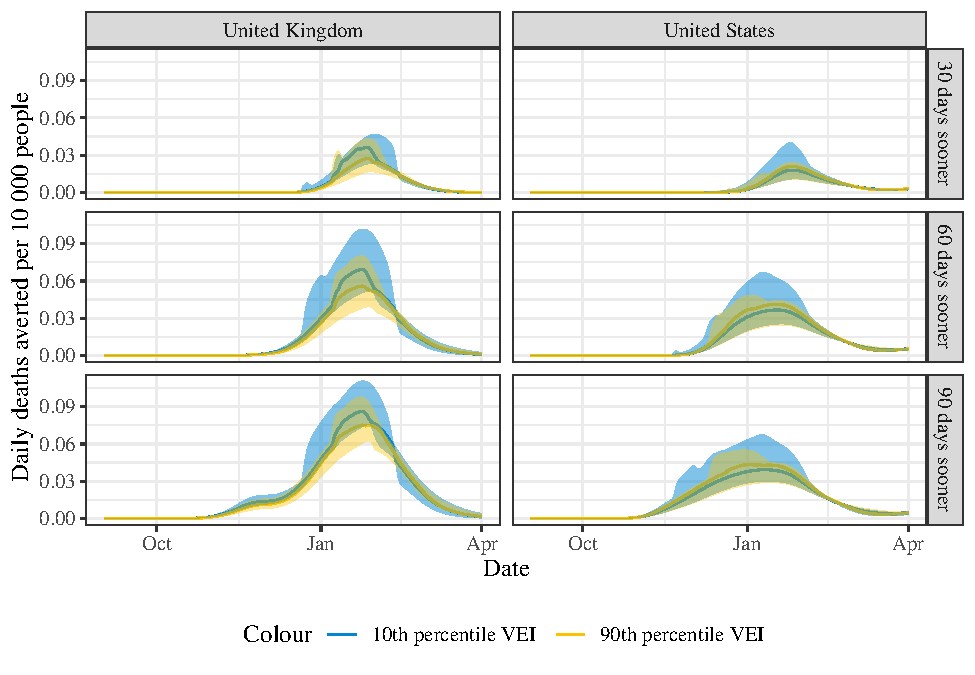
\includegraphics[height=0.35\textheight,]{_main_files/figure-latex/deaths-averted-plot-vei-1}

}

\caption{Daily averted deaths under counterfactual scenarios, with sensitivity to vaccine efficacy. Shaded area indicates 95\% confidence interval.}\label{fig:deaths-averted-plot-vei}
\end{figure}
\begin{figure}[H]

{\centering 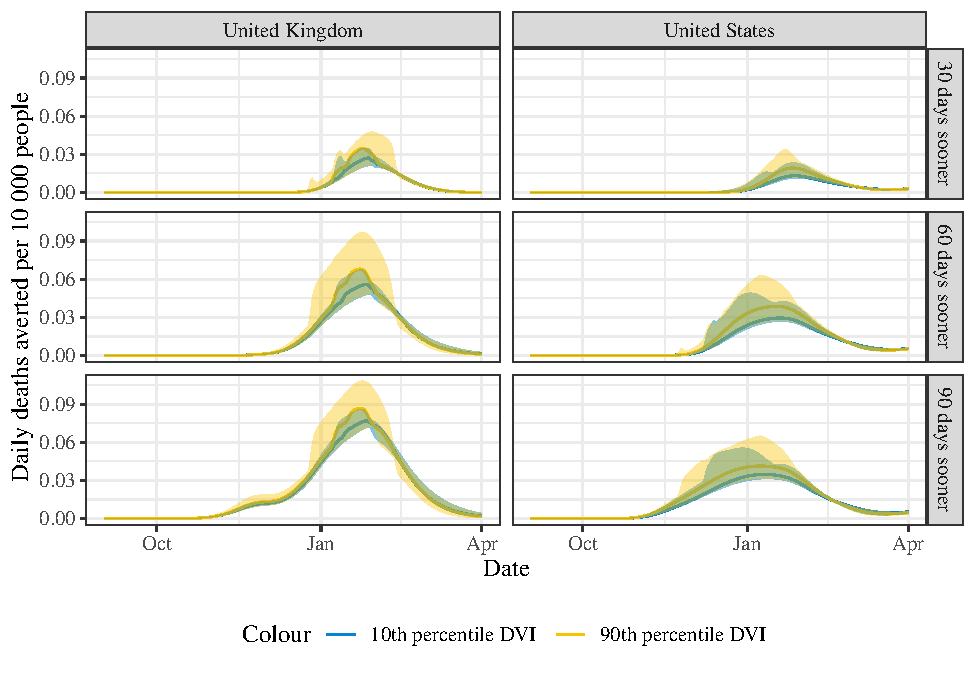
\includegraphics[height=0.35\textheight,]{_main_files/figure-latex/deaths-averted-plot-durV-1}

}

\caption{Daily averted deaths under counterfactual scenarios, with sensitivity to vaccine duration. Shaded area indicates 95\% confidence interval.}\label{fig:deaths-averted-plot-durV}
\end{figure}
\begin{figure}[H]

{\centering 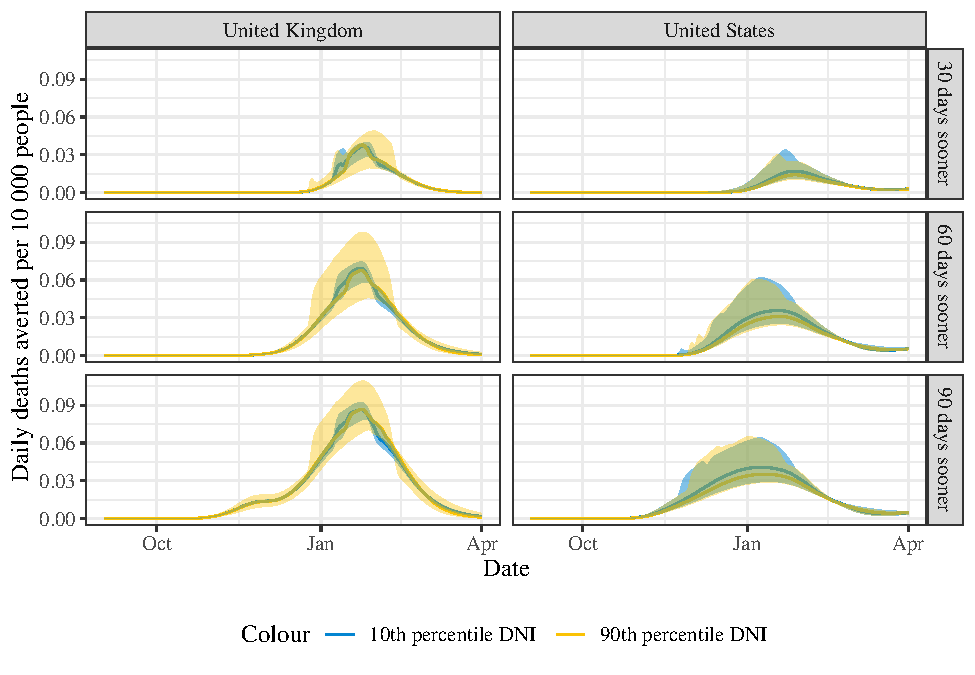
\includegraphics[height=0.35\textheight,]{_main_files/figure-latex/deaths-averted-plot-durR-1}

}

\caption{Daily averted deaths under counterfactual scenarios, with sensitivity to natural immunity duration. Shaded area indicates 95\% confidence interval.}\label{fig:deaths-averted-plot-durR}
\end{figure}
\begin{figure}[H]

{\centering 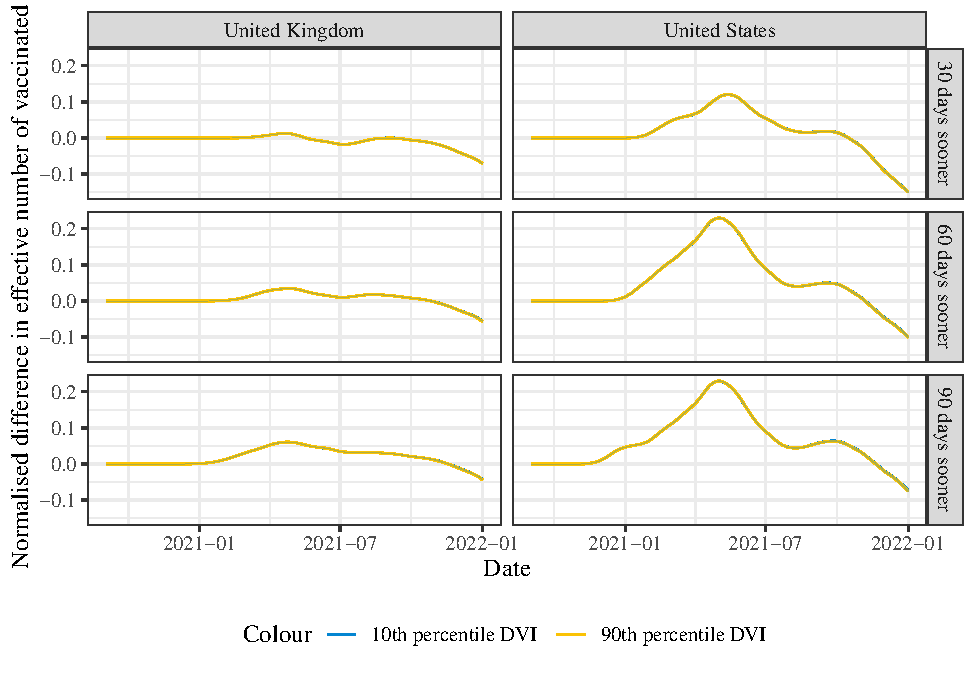
\includegraphics[height=0.35\textheight,]{_main_files/figure-latex/vaccinated-plot-vei-1}

}

\caption{Effective vaccinated, sensitivity to vaccine duration}\label{fig:vaccinated-plot-vei}
\end{figure}

\end{document}
